\documentclass[11pt]{article}
\usepackage[margin=1.2in]{geometry}
\usepackage{amsmath, amssymb, amsthm}
\usepackage{natbib}
\usepackage{hyperref}
\usepackage{booktabs}
\usepackage{graphicx}
\usepackage{tikz}
\usetikzlibrary{shapes, arrows, positioning}
\usepackage{xcolor}
\definecolor{copper}{RGB}{143, 62, 34}
\hypersetup{colorlinks=true, linkcolor=copper, citecolor=copper, urlcolor=copper}

% Theorem environments
\newtheorem{theorem}{Theorem}
\newtheorem{proposition}{Proposition}
\newtheorem{definition}{Definition}
\newtheorem{remark}{Remark}

\title{\textbf{Applied Life: Intelligence Meets Living Systems}\\
{\large AI $\times$ Biology --- Foundation Models, Protein Design, Perturbation Biology,\\and the Causal Frontier}}
\author{Thursday Learning Hours --- TLH-2\\Prabakaran Chandran}
\date{2026}

\begin{document}

\maketitle
\begin{abstract}
We are in the foundation model era for biology. AlphaFold solved protein structure prediction and won a Nobel Prize. Evo 2 reads 9 trillion DNA base pairs across all domains of life. GenBio AI's AIDO spans the entire biological hierarchy from nucleotide to cell. These systems predict biological properties with unprecedented accuracy --- yet every one is causally opaque. This report surveys the AI+Biology landscape across six problem spaces: (1) biological foundation models, (2) protein design and engineering, (3) perturbation biology and drug discovery, (4) causal and mechanistic understanding, (5) synthetic biology, and (6) computational neuroscience. We argue that the open frontier is not better prediction but causal understanding: representations that provably correspond to real biological mechanisms. Biology is uniquely positioned to advance this frontier --- CRISPR perturbations are genuine do-interventions on the biological causal graph, providing exactly the interventional data that causal representation learning (CRL) identifiability theorems require. The marriage of biological foundation models and CRL theory is the deepest open problem in the field.
\end{abstract}

\tableofcontents
\newpage

\section{Introduction}

Biology is the ultimate complex system. It is hierarchical, multi-scale, interventional, and causally structured. The progression from DNA to RNA to protein to cell to tissue represents a cascade of information transformation, each level governed by causal mechanisms that evolution has refined over billions of years.

For decades, computational biology operated at the margins of this complexity --- limited by data, compute, and models. The period from 2020 to 2026 changed this entirely. AlphaFold 2 \citep{jumper2021highly} solved the 50-year protein structure prediction problem at CASP14, achieving near-experimental accuracy on unseen protein sequences and earning the Nobel Prize in Chemistry in 2024. Evo 2 \citep{nguyen2024evo2} trained a 7-billion parameter model on 9 trillion DNA base pairs across all domains of life, demonstrating genome-scale understanding with a 1-million-token context window. GenBio AI's AIDO system \citep{xing2025aido} connects foundation models at every biological scale --- DNA, RNA, protein, cell, and tissue --- creating the first AI system that mirrors the actual hierarchical causal structure of biology.

Yet every one of these systems predicts without understanding. They are extraordinarily powerful pattern matchers over biological sequences, trained by evolution's implicit supervision signal. But none provides guarantees that learned representations correspond to true biological mechanisms. This is the causal gap.

This report maps the AI+Biology landscape, identifies the key problem spaces, surveys the state of the art, and argues that causal representation learning \citep{scholkopf2021toward} provides the missing theoretical lens. Perturbation biology --- CRISPR knockouts combined with single-cell transcriptomics --- provides the interventional data CRL requires. The union of these fields is the frontier.

\section{The Biological Hierarchy as a Data Problem}

Biology is organized in a hierarchy of scales, each with distinct data modalities and ML challenges:

\begin{table}[h]
\centering
\begin{tabular}{lllll}
\toprule
\textbf{Scale} & \textbf{Data Type} & \textbf{Dimensionality} & \textbf{Key Technology} & \textbf{ML Problem} \\
\midrule
DNA & Nucleotide sequence & $3 \times 10^9$ bp (human) & Next-gen sequencing & Sequence modeling \\
RNA & Expression profile & $\sim 20{,}000$ genes & RNA-seq / scRNA-seq & Expression modeling \\
Protein & AA sequence + 3D & $\sim 100$--3,000 AAs & Cryo-EM / X-ray & Seq + structure pred. \\
Cell & Transcriptomic state & $\sim 20{,}000$ genes & 10X Genomics & State modeling \\
Tissue & Spatial + expression & $\sim 10^6$ cells & Visium / MERFISH & Spatial modeling \\
\bottomrule
\end{tabular}
\caption{The biological hierarchy as a machine learning problem. Each scale presents natural sequence or vector structures amenable to transformer architectures.}
\end{table}

\subsection{The Central Dogma as a Causal Chain}

The central dogma of molecular biology states: DNA $\rightarrow$ RNA $\rightarrow$ Protein. This is a \emph{causal} chain, not merely a correlational one. DNA sequence determines which proteins can be made; RNA mediates the information transfer; proteins execute biological function. Regulation operates at every step, creating a complex causal graph.

\begin{definition}[Biological Causal Graph]
Let $\mathcal{G} = (\mathcal{V}, \mathcal{E})$ be a directed acyclic graph where nodes represent biological entities (genes, proteins, metabolites, cells) and edges represent causal regulatory relationships. The observed biological state $\mathbf{X}$ is generated by:
$$\mathbf{X}_i = f_i(\mathbf{X}_{\mathrm{Pa}(i)}, \epsilon_i)$$
where $\mathrm{Pa}(i)$ are the causal parents of node $i$ in $\mathcal{G}$ and $\epsilon_i$ is independent noise.
\end{definition}

This structural causal model (SCM) formulation \citep{pearl2009causality} is the natural language for biology. The entire program of systems biology --- understanding gene regulatory networks, signaling pathways, and metabolic circuits --- is the program of learning $\mathcal{G}$ from data.

\subsection{The Perturbation Paradigm}

CRISPR-Cas9 gene editing enables precise interventions in the biological causal graph. A gene knockout corresponds exactly to the \emph{do}-operation of Pearl's do-calculus: $do(X_i = 0)$ sets gene $i$ to zero regardless of its upstream regulators.

Perturb-seq \citep{dixit2016perturb} combines CRISPR knockouts with single-cell RNA sequencing at scale. Replogle et al. \citep{replogle2022mapping} performed genome-scale Perturb-seq: 9,000+ gene knockouts across 2.5 million cells in K562 human leukemia cells. This is the largest systematic collection of biological do-interventions ever assembled.

\begin{remark}
Perturb-seq data is unique in the ML landscape: it provides paired observational data $P(\mathbf{X})$ and interventional data $P(\mathbf{X} \mid do(X_i = 0))$ for thousands of interventions $i$. This is exactly the multi-environment interventional setting required for causal representation learning identifiability.
\end{remark}

\section{Foundation Models for Biology}

\subsection{Protein Language Models: ESM-2}

Lin et al. \citep{lin2023evolutionary} trained ESM-2, a masked language model on 250 million UniRef90 protein sequences. The key insight is that protein sequences encode 3D structure implicitly through evolutionary co-variation: amino acid pairs that are in spatial contact tend to co-evolve, because mutations at one position must be compensated by mutations at the other to maintain function.

ESM-2 learns to predict masked amino acids from context, which forces the model to internalize the structural and functional constraints encoded in evolutionary sequence variation. The result:

\begin{proposition}[Emergent Structure Prediction]
ESM-2 representations at the 33-layer, 650M parameter scale predict amino acid contacts (3D proximity) at $\sim$0.7 precision on unseen proteins, without any structural supervision during training. The representations have intrinsic structural geometry.
\end{proposition}

ESMFold extends ESM-2 to direct structure prediction using only the protein sequence as input, achieving AlphaFold2-class accuracy at $60\times$ lower computational cost.

\subsection{Genome-Scale Models: Evo 2}

Nguyen et al. \citep{nguyen2024evo2} (Arc Institute) trained Evo 2 on 9 trillion DNA base pairs spanning bacteria, archaea, and eukaryotes --- the most comprehensive genomic training corpus assembled. A 1-million-token context window enables the model to process entire bacterial genomes at single-nucleotide resolution.

Evo 2 capabilities:
\begin{enumerate}
\item Predict the effect of any single-nucleotide variant on gene function
\item Generate novel protein-coding DNA sequences with desired properties
\item Design functional CRISPR guide RNAs targeting any genomic locus
\item Understand long-range regulatory elements spanning megabase distances
\end{enumerate}

\subsection{AIDO: The Multi-Scale Foundation Model System}

Xing et al. \citep{xing2025aido} (GenBio AI) introduce AIDO --- AI-Driven Digital Organism --- a system of connected foundation models spanning the biological hierarchy. AIDO differs from all prior biological FMs in architecture philosophy: rather than training a single model on mixed biological data, AIDO trains modular, scale-specific FMs that are then connected to reflect the actual causal structure of biology.

\begin{center}
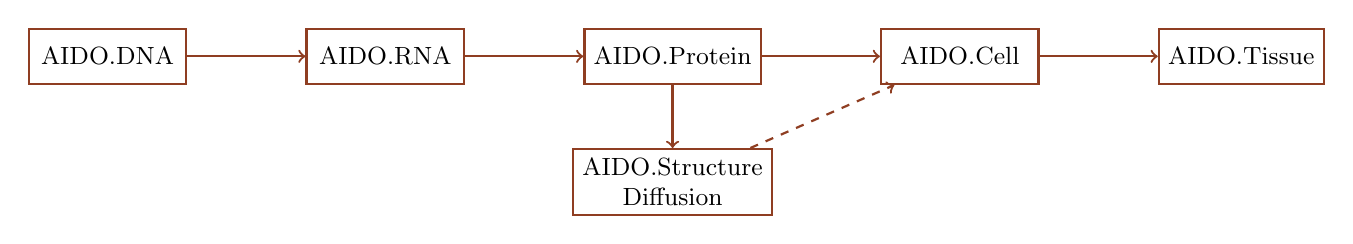
\begin{tikzpicture}[
  box/.style={rectangle, draw=copper, thick, minimum width=2cm, minimum height=0.7cm, align=center, font=\small},
  arr/.style={->, thick, draw=copper}
]
\node[box] (dna) {AIDO.DNA};
\node[box, right=1.5cm of dna] (rna) {AIDO.RNA};
\node[box, right=1.5cm of rna] (prot) {AIDO.Protein};
\node[box, right=1.5cm of prot] (cell) {AIDO.Cell};
\node[box, right=1.5cm of cell] (tissue) {AIDO.Tissue};
\node[box, below=0.8cm of prot] (struct) {AIDO.Structure\\Diffusion};
\draw[arr] (dna) -- (rna);
\draw[arr] (rna) -- (prot);
\draw[arr] (prot) -- (cell);
\draw[arr] (cell) -- (tissue);
\draw[arr] (prot) -- (struct);
\draw[arr, dashed] (struct) -- (cell);
\end{tikzpicture}
\end{center}

AIDO achieves state-of-the-art on 300+ biological tasks across all scales. AIDO.Cell enables virtual cell simulation: given a cell type and a perturbation, predict the resulting gene expression profile.

\section{Protein Design and Engineering}

\subsection{From Prediction to Generation}

AlphaFold 2 \citep{jumper2021highly} established that protein structure is predictable from sequence with near-experimental accuracy. The field has since moved from prediction to \emph{design}: given a desired function or binding target, generate a protein sequence that achieves it.

The full protein design pipeline:

\begin{enumerate}
\item \textbf{Backbone design (RFdiffusion):} Watson et al. \citep{watson2023novo} trained a diffusion model over protein backbone coordinates, conditioned on desired properties (symmetry, binding sites, functional motifs). Given a target, RFdiffusion generates diverse 3D backbone scaffolds.

\item \textbf{Sequence design (ProteinMPNN):} Dauparas et al. \citep{dauparas2022robust} trained ProteinMPNN for inverse folding --- given a 3D backbone, design an amino acid sequence that will fold into it. ProteinMPNN generates millions of candidate sequences per backbone.

\item \textbf{Structure validation (AlphaFold 3):} Evans et al. \citep{evans2024alphafold3} extended AF2 to predict interactions between proteins, DNA, RNA, ligands, and ions. The self-consistency check: run AF3 on the designed sequence; if the predicted structure matches the design intention, the sequence is a viable candidate.

\item \textbf{Fitness ranking (ESM-2):} Use ESM-2 log-likelihood as a zero-shot fitness predictor to rank and filter candidates before wet lab synthesis.
\end{enumerate}

\subsection{The Fitness Landscape Problem}

A protein's function can be represented as a fitness landscape $f: \mathcal{A}^L \rightarrow \mathbb{R}$ mapping sequences (over alphabet $\mathcal{A}$ of 20 amino acids) to fitness scores. The landscape is high-dimensional ($L \sim 100$--3,000), non-convex, and epistatic (mutations interact).

\begin{definition}[Epistasis]
A mutation $m_i$ at position $i$ is epistatic with mutation $m_j$ at position $j$ if:
$$f(\mathbf{x} + m_i + m_j) \neq f(\mathbf{x} + m_i) + f(\mathbf{x} + m_j) - f(\mathbf{x})$$
The fitness effect of $m_i$ depends on whether $m_j$ is also present.
\end{definition}

Epistasis is ubiquitous in proteins --- the same mutation that is deleterious in one background is beneficial in another. This makes fitness landscape navigation fundamentally combinatorial and motivates the AI approaches surveyed here.

\section{Perturbation Biology and the CRL Frontier}

\subsection{The Core Task}

Given a cell type $C$ and a perturbation $P$ (gene knockout, drug treatment), predict the resulting gene expression profile:
$$\hat{\mathbf{x}}_P = \text{Model}(\mathbf{x}_{\text{ctrl}}, P) \approx \mathbf{x}_{P}$$
where $\mathbf{x} \in \mathbb{R}^{n_{\text{genes}}}$ is the gene expression vector.

GEARS \citep{roohani2023gears} is the current state of the art, using a gene interaction knowledge graph (STRING database) and a graph neural network to propagate perturbation effects through the network. GEARS can predict combinatorial perturbation effects --- the response to knocking out two genes simultaneously --- even when only single-gene training data is available.

\subsection{CRL for Biology: Identifiability}

The fundamental question is not accuracy but \emph{causal faithfulness}: do the learned representations correspond to true biological mechanisms?

\begin{definition}[Causal Faithfulness of Biological Representations]
A model $\phi$ learning latent representation $\mathbf{z} = \phi(\mathbf{x})$ from single-cell data is causally faithful if there exists a bijection $\sigma$ such that $\mathbf{z}_i = \sigma(\mathbf{c}_i)$, where $\mathbf{c}$ are the true latent biological causal factors (cell type, signaling state, stress response, etc.).
\end{definition}

Sun, Zhang, and Xing \citep{sun2025crl} (ICLR 2025) prove identifiability conditions for CRL from multimodal biomedical observations --- the direct theoretical bridge between CRL theory and biological data. The key condition: interventions (perturbations) must change sparse subsets of causal mechanisms independently.

\begin{theorem}[Informal, from Sun et al. 2025]
Under mild regularity conditions, if single-cell perturbation data is collected across multiple cell types and perturbation conditions such that each perturbation shifts a sparse, distinct subset of causal mechanisms, then the latent biological causal factors are identifiable (up to permutation and component-wise transformation) from the observational + interventional data.
\end{theorem}

This theorem is powerful because Perturb-seq data is precisely multi-condition, multi-perturbation single-cell data with sparse interventions. The biological problem maps cleanly onto the mathematical requirements.

\subsection{The Open Research Program}

The open questions that define the frontier:
\begin{enumerate}
\item Do AIDO.Cell's learned representations of cell state satisfy the causal faithfulness condition?
\item What specific intervention design (single knockouts? combinatorial? dosage sweeps?) provides the richest identifiability signal?
\item Can we design a falsifiable test for causal faithfulness of biological FM representations?
\item How does the CRL identifiability framework extend to the full biological hierarchy (DNA → Cell)?
\end{enumerate}

\section{Drug Discovery}

Stokes et al. \citep{stokes2020deep} demonstrated that AI could discover functionally novel antibiotics (halicin) by screening 107 million molecular candidates in silico. This paper established the template: train a property predictor on a small labeled dataset, apply it to a vast chemical library, synthesize top-scoring candidates.

The field has since moved from single-property prediction to multi-objective optimization over ADMET properties (absorption, distribution, metabolism, excretion, toxicity) and target binding simultaneously. Isomorphic Labs' IsoDDE (2026) --- the successor to AlphaFold 3 --- predicts binding affinities and identifies novel binding pockets at scale, promising to compress the lead optimization phase from years to weeks.

\section{Outlook}

The AI+Biology field is moving at unprecedented speed. Key predictions for the next 3 years:
\begin{enumerate}
\item \textbf{Causal bio FMs} will emerge --- models trained with explicit interventional supervision from Perturb-seq data, providing identifiable representations
\item \textbf{Virtual cells} will become standard evaluation environments --- replacing or augmenting wet lab assays for initial screening
\item \textbf{Protein design success rate} will reach 50\%+ for de novo binders --- making designed proteins a standard tool in biology
\item \textbf{Drug discovery timelines} will compress from 12+ years to 5--7 years as AI handles the first 3 phases in silico
\item \textbf{CRL × bio} will become a major subfield at NeurIPS, ICLR, and Nature Methods
\end{enumerate}

\section*{Acknowledgments}
Thursday Learning Hours initiative, PraCha Labs. References to pre-reads and resources compiled from the Applied Life pillar landscape survey.

\bibliographystyle{abbrvnat}
\begin{thebibliography}{99}

\bibitem{jumper2021highly}
Jumper, J., et al. (2021). Highly accurate protein structure prediction with AlphaFold. \textit{Nature}, 596, 583--589.

\bibitem{nguyen2024evo2}
Nguyen, E., et al. (2024). Evo 2: DNA foundation models from genomes to molecules. \textit{Nature}.

\bibitem{xing2025aido}
Xing, E., et al. (2025). AIDO: A foundation model system spanning the molecular and cellular hierarchy of life. \textit{GenBio AI Technical Report}.

\bibitem{lin2023evolutionary}
Lin, Z., et al. (2023). Evolutionary-scale prediction of atomic-level protein structure with a language model. \textit{Science}, 379, 1123--1130.

\bibitem{watson2023novo}
Watson, J. L., et al. (2023). De novo design of protein structure and function with RFdiffusion. \textit{Nature}, 620, 1089--1100.

\bibitem{dauparas2022robust}
Dauparas, J., et al. (2022). Robust deep learning--based protein sequence design using ProteinMPNN. \textit{Science}, 378, 49--56.

\bibitem{evans2024alphafold3}
Evans, R., et al. (2024). Accurate structure prediction of biomolecular interactions with AlphaFold 3. \textit{Nature}, 630, 493--500.

\bibitem{roohani2023gears}
Roohani, Y., et al. (2023). GEARS: Predicting transcriptional outcomes of novel multi-gene perturbations. \textit{Nature Biotechnology}, 42, 927--935.

\bibitem{norman2019exploring}
Norman, T. M., et al. (2019). Exploring genetic interaction manifolds constructed from rich single-cell phenotypes. \textit{Science}, 365, 786--793.

\bibitem{replogle2022mapping}
Replogle, J. M., et al. (2022). Mapping information-rich genotype--phenotype landscapes with genome-scale Perturb-seq. \textit{Cell}, 185, 2559--2575.

\bibitem{dixit2016perturb}
Dixit, A., et al. (2016). Perturb-seq: Dissecting molecular circuits with scalable single-cell RNA profiling of pooled genetic screens. \textit{Cell}, 167, 1853--1866.

\bibitem{scholkopf2021toward}
Schölkopf, B., et al. (2021). Toward causal representation learning. \textit{Proceedings of the IEEE}, 109, 612--634.

\bibitem{sun2025crl}
Sun, Y., Zhang, K., Xing, E., et al. (2025). Causal representation learning from multimodal biomedical observations. \textit{ICLR 2025}.

\bibitem{pearl2009causality}
Pearl, J. (2009). \textit{Causality: Models, Reasoning, and Inference} (2nd ed.). Cambridge University Press.

\bibitem{stokes2020deep}
Stokes, J. M., et al. (2020). A deep learning approach to antibiotic discovery. \textit{Cell}, 180, 688--702.

\bibitem{theodoris2023geneformer}
Theodoris, C. V., et al. (2023). Transfer learning enables predictions in network biology. \textit{Nature}, 618, 616--624.

\bibitem{cui2024scgpt}
Cui, H., et al. (2024). scGPT: toward building a foundation model for single-cell multi-omics using generative AI. \textit{Nature Methods}, 21, 1470--1480.

\bibitem{lotfollahi2019scgen}
Lotfollahi, M., et al. (2019). Predicting single-cell perturbations with deep learning. \textit{Nature Methods}, 16, 715--721.

\bibitem{lopez2018scvi}
Lopez, R., et al. (2018). Deep generative modeling for single-cell transcriptomics. \textit{Nature Methods}, 15, 1053--1058.

\end{thebibliography}

\end{document}
